\documentclass[11pt,letterpaper]{article}
\usepackage{graphicx} %
\usepackage{subcaption}
\usepackage[letterpaper, margin=0.9in]{geometry}

\usepackage{xcolor}
\usepackage{amsmath}
\usepackage{amsthm}
\usepackage[hyphens]{url}
\usepackage[breaklinks=true]{hyperref}
\usepackage{titlesec}

\usepackage{authblk}


\usepackage{floatrow}
\usepackage{epigraph}
\setlength{\epigraphwidth}{0.4\textwidth}

\usepackage{algorithm}
\usepackage{algpseudocode}

\usepackage{xparse}
\ExplSyntaxOn
\int_new:N \g_my_cycle_int
\seq_new:N \g_my_items_seq
\NewDocumentCommand{\setcycle}{m}
 {
  \seq_set_from_clist:Nn \g_my_items_seq { #1 }
  \int_gset:Nn \g_my_cycle_int { 0 }
 }
\NewDocumentCommand{\venn}{}
 {
  \int_gadd:Nn \g_my_cycle_int { 1 }
  \int_compare:nNnT { \g_my_cycle_int } > { \seq_count:N \g_my_items_seq }
   { \int_gset:Nn \g_my_cycle_int { 1 } }
  \seq_item:Nn \g_my_items_seq { \g_my_cycle_int }
 }
\ExplSyntaxOff
\setcycle{{Ven diagram}, {Venne diagram}, {Venn digram}, {Venn diagrame}, {Venn diagramm}, {Vin diagram}, {Vennn diagram}, {venn diagram}, {Ben diagram}, {Venn-diagram}, {Vann diagram}, {Euler diagram}}

\pdfstringdefDisableCommands{%
    \def\pie{}%
}

\usepackage{fontspec} %
\newcommand{\pie}{{\fontspec{Symbola}\char"1F967}}


\title{\pie{} is all you eat}
\author{Markus Reiter-Haas, Kevin Innerebner}
\affil{\pie{} for Society Lab}
\date{February 2026}

\newcommand{\todo}[1]{
    \textcolor{red}{\textbf{/* TODO: #1 */}}
}

\renewcommand{\topfraction}{0.4}

\begin{document}



\maketitle
\thispagestyle{empty}
\pagestyle{empty}

\begin{abstract}
    \pie{} is love, \pie{} is life -- \pie{} is all you eat!

\begin{figure}[h]
    \centering
    \makebox[\textwidth][c]{%
    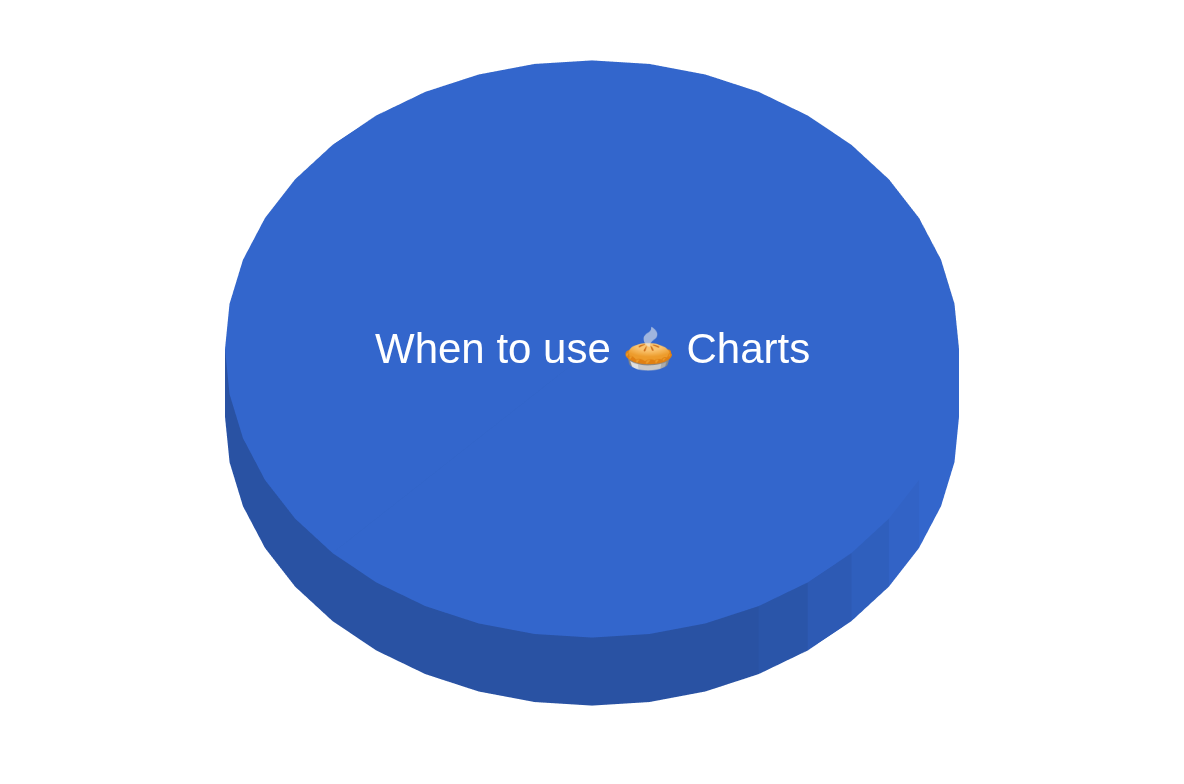
\includegraphics[width=1.3\textwidth]{pie_charts/pie1_fig1.png}
    }
    \caption{Visual Abstract that shows when to use \pie{}charts.}
    \label{fig:pie}
\end{figure}
\end{abstract}


\section{Introduction (or \pie{} for dummies)}
\epigraph{Let them eat \pie{}!}{}
\noindent
Effective data visualization is considered challenging, as people often ponder which type of visualization to use. Some visualizations cram too much information into one chart, making them confusing. Besides, this leads to less paper space being used for visualizations, which in turn requires people to write more words to meet the space limit in a report, hampering productivity. The charts also often have irregular shapes where most of the space does not use up any ink when printing. To combat this temporal and spatial wastefulness, we argue that more \pie{} is needed, which is not only delicious but is also a nutritious source for carbs (see Figure~\ref{fig:pienutrtion}). The high calorie density of \pie{}\pie{} makes them a beloved staple in the nutrition of billions of people. We believe that \pie{}charts have a similar appeal to transform science due to their information-theoretic efficiency, i.e.,  using up paper space in relation to bits of information. To that end, we introduce \pie{}viz, a \pie{}thon library for all your future data visualizations. \pie{}viz allows for engaging, \pie{}-driven storytelling in academic papers, while fostering food cravings in readers --- directly increasing the real-world impact of the paper.

\begin{figure}[h]
    \centering
    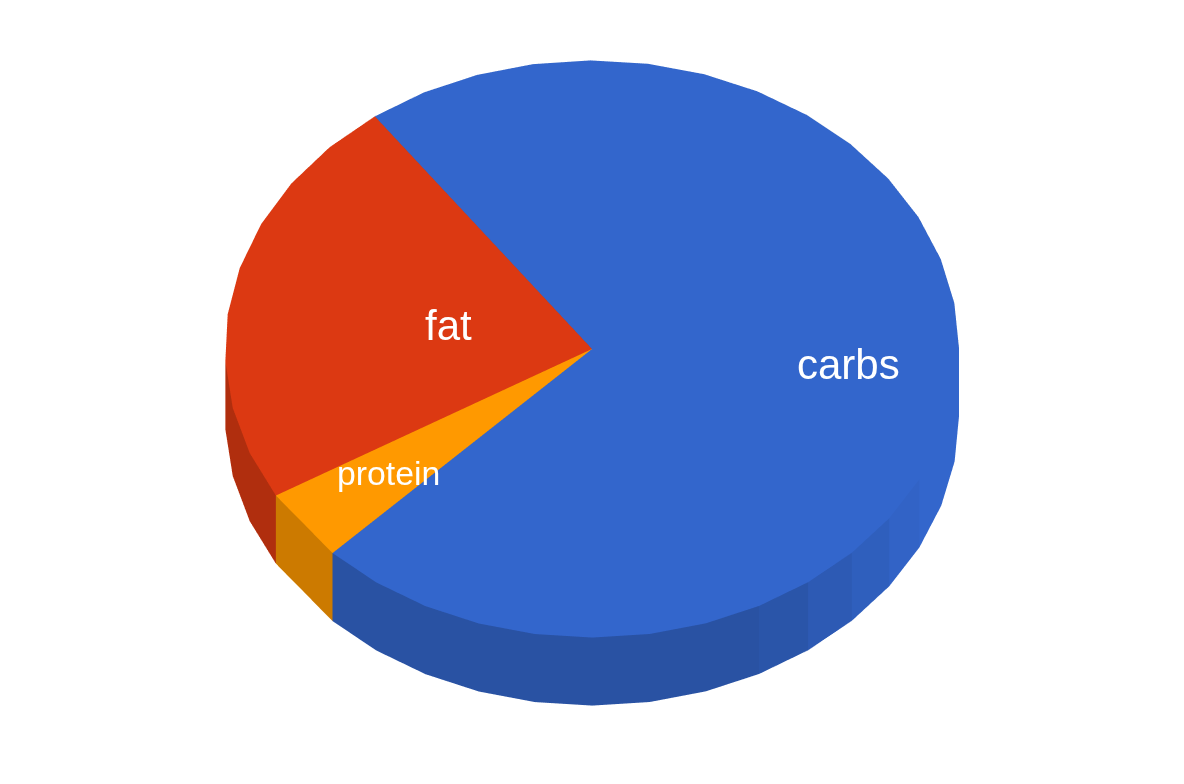
\includegraphics[width=0.5\linewidth]{pie_charts/pie2_nutri_stats.png}
    \caption{\pie{} is a rich source of carbs to balance the high amount of protein often found in other food. Estimation for apple \pie{}.}
    \label{fig:pienutrtion}
\end{figure}

As most businesspeople already know, but which remains relatively unknown to academics: \pie{}charts are superior to \emph{all} other data visualizations in \emph{every} scenario. This paper investigates the reasons for this superiority by addressing the important research question of \textbf{``Why are \pie{}charts superior?''}.


\section{Unrelated Work in Data Visualizations (w/o \pie{}\pie{})}
\epigraph{as easy as \pie{}}{}
\noindent
Several data visualizations have been proposed over the years. Some of them try to tackle the shortcomings of others. For instance, UpSet plots~\cite{lex2014upset} provide an alternative to \venn{}s for intersecting sets. We believe that this effort was \textbf{wasted}, as \pie{}charts already provided the best alternative. Some data visualization researchers might claim that's like comparing an apple \pie{} to a pear \pie{} (yummy). However, we find that a series of \pie{}chart is much more sufficient even in that scenario. Consider blood types, which are typically visualized as a single \venn{} but can quickly be done with a series of \pie{}charts (see Figure~\ref{fig:venn}). \pie{}charts also approximately preserve ratios while being entirely agnostic to the magnitude of the data. Hence, it does not matter if your data is off by a bit and there are no scaling issues with very large numbers, as the size of the whole \pie{} remains the same.

\begin{figure}[t]
    \centering
    \begin{subfigure}[t]{0.33\textwidth}
        \centering
        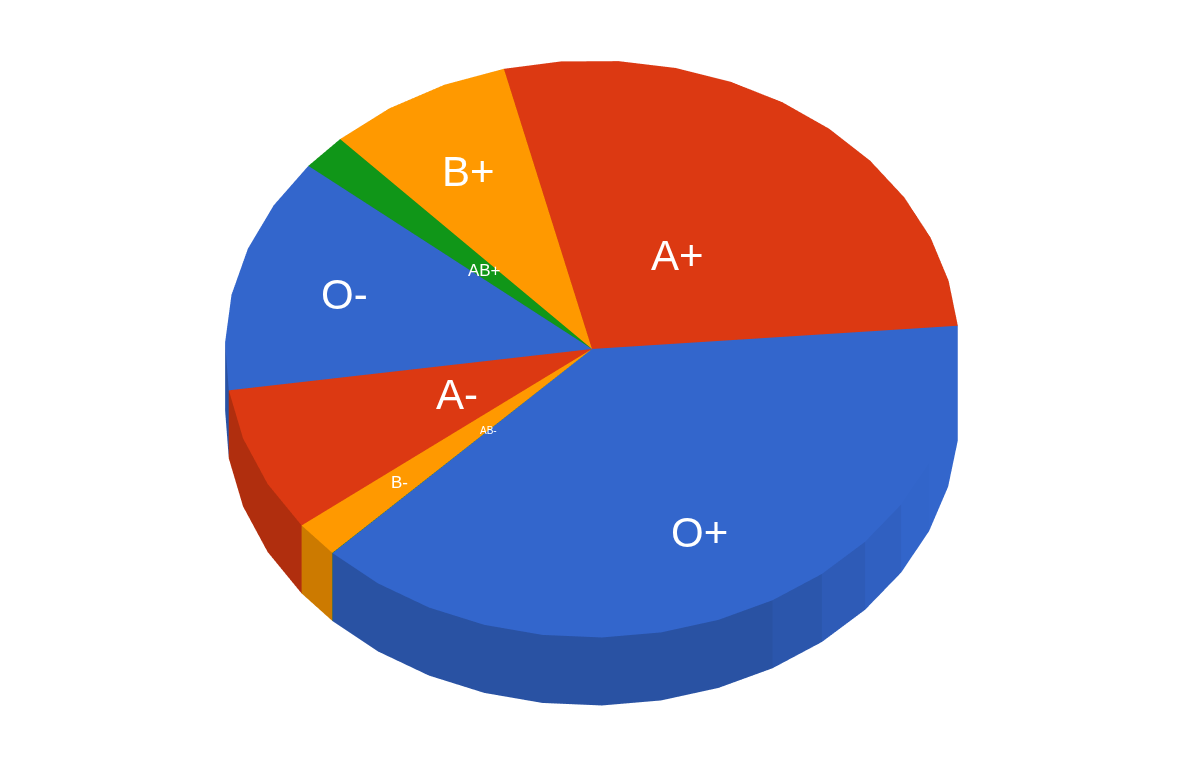
\includegraphics[width=\linewidth]{pie_charts/pie3_blood.png}
        \caption{Blood type distribution}
    \end{subfigure}%
    \hfill
    \begin{subfigure}[t]{0.33\textwidth}
        \centering
        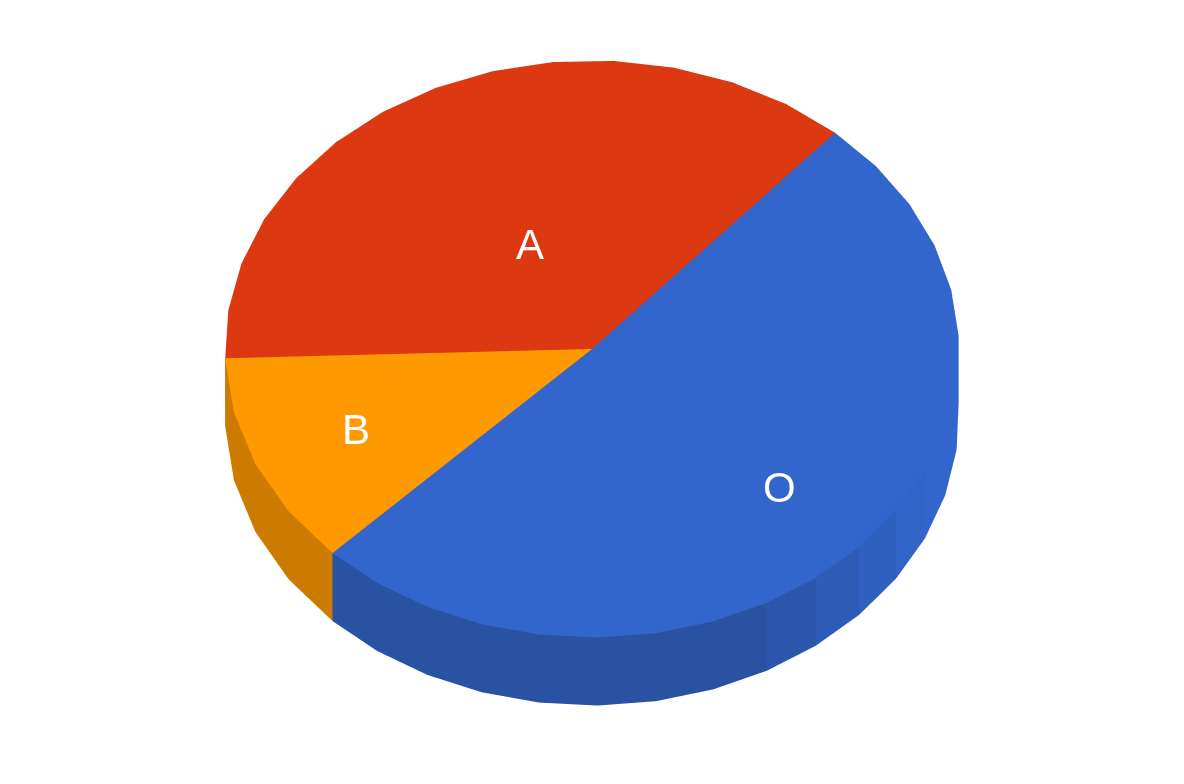
\includegraphics[width=\linewidth]{pie_charts/pie3_ABO.png}
        \caption{ABO distribution}
    \end{subfigure}%
    \hfill
    \begin{subfigure}[t]{0.33\textwidth}
        \centering
        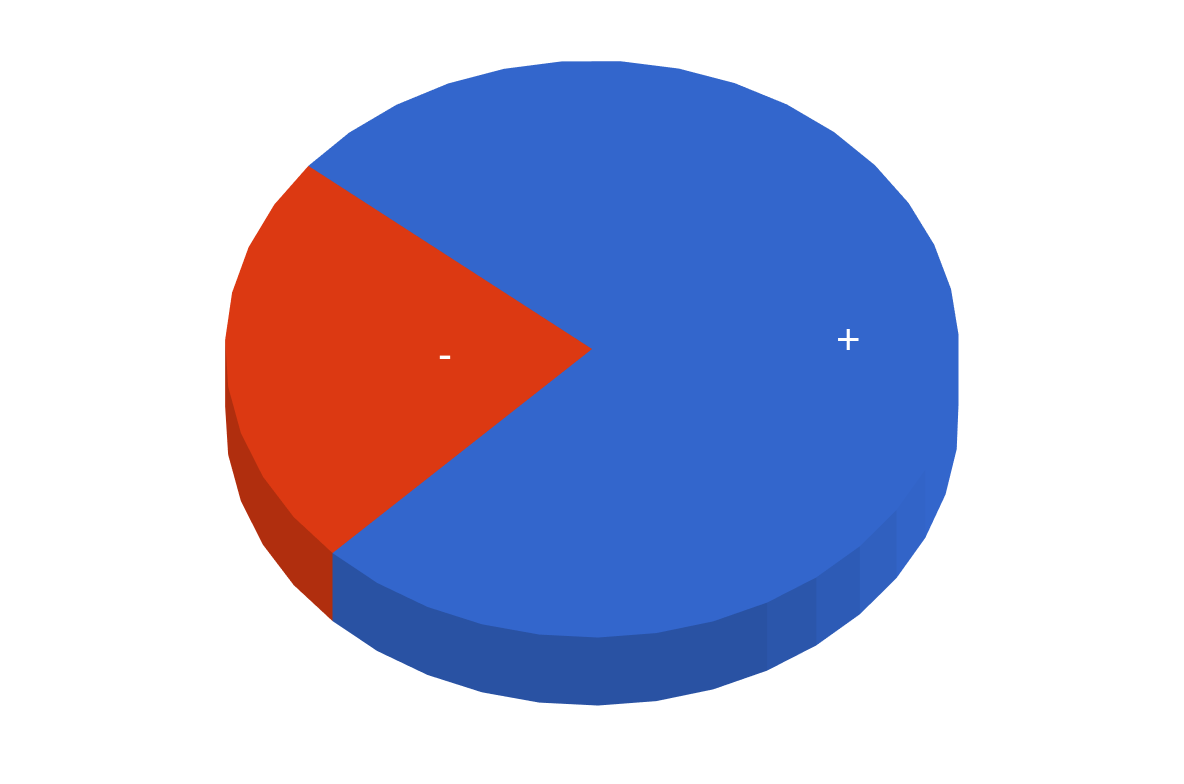
\includegraphics[width=\linewidth]{pie_charts/pie3_Rh.png}
        \caption{Rh distribution}
    \end{subfigure}%
    \caption{\pie charts to visualize intersecting sets. }
    \label{fig:venn}
\end{figure}

\noindent
To be  more specific, we find several shortcomings in data visualization like UpSet plots~\cite{lex2014upset}:
\begin{enumerate}
    \item their name is often quite UpSetting \ldots
    \item their lack of color and 3D effects in commonly used settings
    \item they require formal training to understand, rendering them unusable for businesspeople
    \item they have high cognitive load requirements due to multiple variables smooshed together into one visualization
    \item they do not efficiently use up paper space and ink
    \item they depend on precise numbers; e.g., bars tend to have vastly different lengths as the magnitude of variables changes (e.g., double length with twice the data)
    \item they do not have rotational invariance
    \item they are not normalized and look very different when the underlying data differs; a \pie{}chart always fills the whole \pie{} and is therefore inherently normalized 
    \item most crucially, these visualizations do not resemble a \pie{} at all!
\end{enumerate}

\noindent
In sum, this clearly demonstrates the advantage of \pie{}-based charts compared to all other types of visualizations. Note that to avoid promoting non-\pie{}-inclusive visualizations, we  refrained from reproducing these inferior visualizations and did not consider any further types of visualization for comparison. This choice enables a streamlined story guided exclusively by \pie{}charts.


\section{Dough Base of \pie{}chart Superiority}
\epigraph{say good\pie{} to other visualizations!}{}
\noindent
In this section, we provide the dough base (aka theoretical underpinnings) on why \pie{}charts are superior. First, we prove how efficiently \pie{}charts can utilize the ink (and therefore space) when printing papers. Second, we investigate the prevalence of \pie{}chart usage compared to \venn{}s and UpSet plots. Third, we conducted a user study, which shows that \pie{}charts are most often identified and receive the most points.

\subsection{Proof of \pie{} Ink Efficiency}
\epigraph{Cut my \pie{} into eight \pie{}ces, I don’t think I could eat sixteen.}{}
\noindent
One objective way to evaluate visualizations is to consider the ink requirements. To that end, we prove the ink and space efficiency of \pie{}charts on various paper formats. We define the ink ratio $I\%$ as the paper space requirements for the visualization --- more is better. For simplicity, we assume boring 2D \pie{}charts. This gives us the following theorem:

\newtheorem{theorem}{Theorem}[section]
\begin{theorem}
Let \(f\) be a paper size with sides \(x\) and \(y\). W.l.o.g. we assume $x<y$. Then a \pie{}chart can use up to I\% of the paper:
\begin{equation}
    I\% = \frac{p(x/2)^2}{(xy)}
\end{equation}
, where $p$ is a constant set to \pie{}. 
\end{theorem}
As we can derive from the equation, for optimal potential ink efficiency, the sides $x$ and $y$ should be as close to each other. We visualize the potential ink efficiency for various paper formats in Figure~\ref{fig:ink}. 

\begin{figure}[h]
    \centering
    \begin{subfigure}[t]{0.25\textwidth}
        \centering
        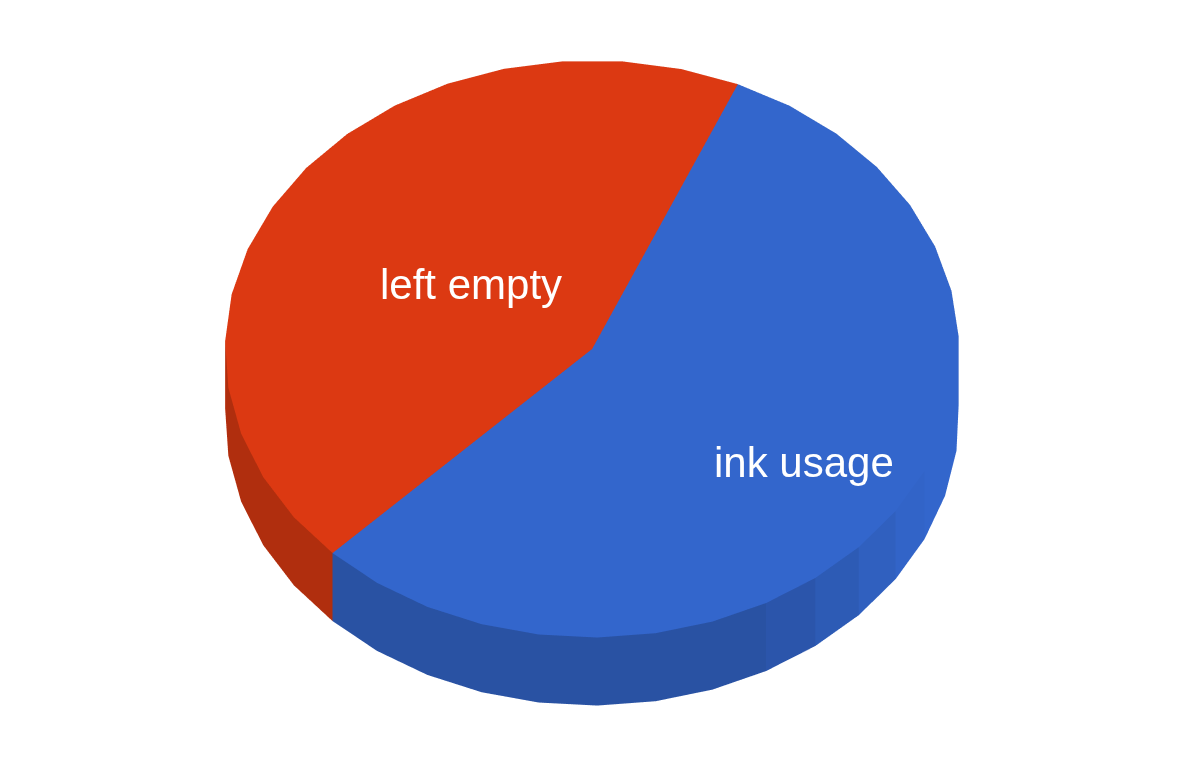
\includegraphics[width=\linewidth]{pie_charts/pie4_A4.png}
        \caption{A4 (DIN 476/ISO 216)}
    \end{subfigure}%
    \hfill
    \begin{subfigure}[t]{0.25\textwidth}
        \centering
        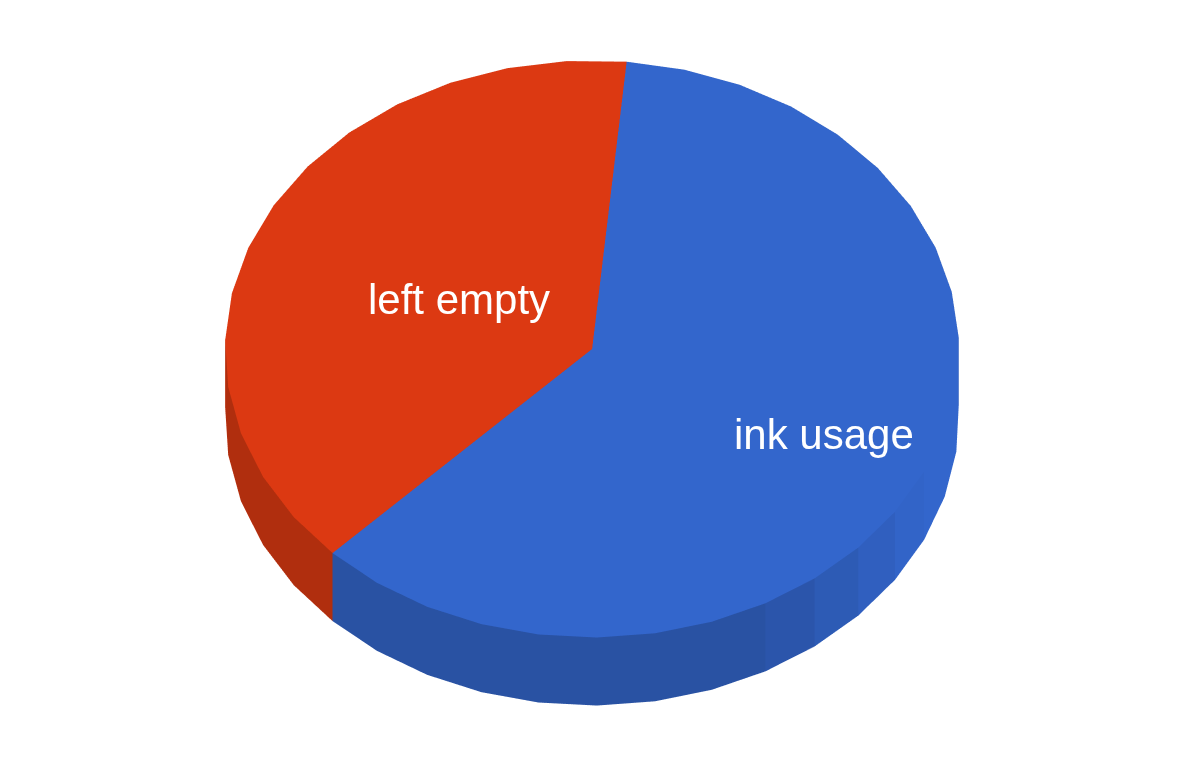
\includegraphics[width=\linewidth]{pie_charts/pie4_US Letter.png}
        \caption{US Letter}
    \end{subfigure}%
    \hfill
    \begin{subfigure}[t]{0.25\textwidth}
        \centering
        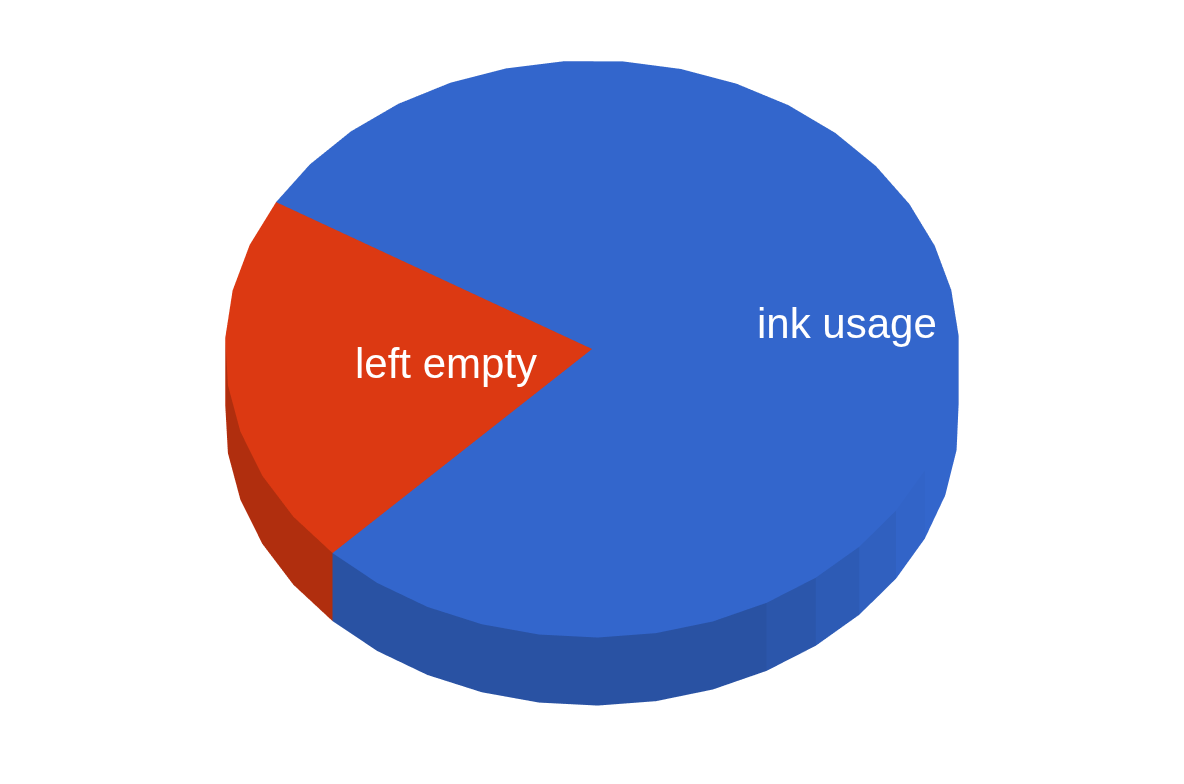
\includegraphics[width=\linewidth]{pie_charts/pie4_Square.png}
        \caption{Square Paper}
    \end{subfigure}%
    \hfill
    \begin{subfigure}[t]{0.25\textwidth}
        \centering
        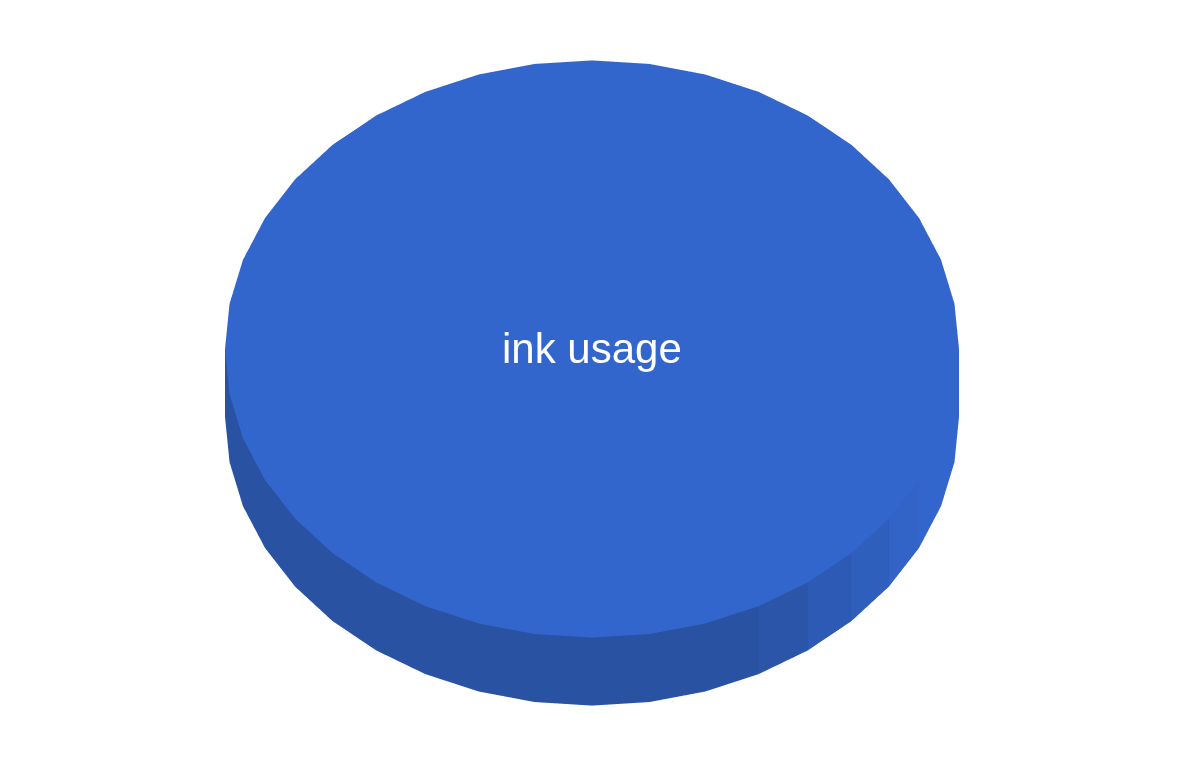
\includegraphics[width=\linewidth]{pie_charts/pie4_Pie Shaped.png}
        \caption{\pie{}-shaped Paper}
    \end{subfigure}%
    \caption{Comparison of paper formats for \pie{} ink efficiency.}
    \label{fig:ink}
\end{figure}

We observe that \pie{}charts could use the majority of any of these paper formats. This fact already shows how ink efficient they are. In comparison, \venn{}s often only use the outline, while UpSet plots tend to even leave gaps between the bars. Due to their irregularity, no exact ink efficiency ratio can be calculated for \venn{}s or UpSet plots. Still, it is evident by inspection that they cannot compete with \pie{}charts regarding ink efficiency $\qedsymbol$.

Concerning the different paper formats, we see that the US letter format can leverage a higher ink efficiency with \pie{}charts. The strong ink efficiency of \pie{}charts on US letters is presumably a strong contributor to the US business performance, where other countries rely on the less optimal ISO standard. Hence, we are pleased that this paper is printed on imperial unit-based paper dimensions. Furthermore, we argue that other formats, like a square paper, would be better. Of course, a \pie{}-shaped paper would allow for optimal ink efficiency, where everything could be used just for the \pie{} visualization. 

Transitioning to efficient paper sizes could also have other positive societal effects, like optimizing printing workload. This would prevent printers from being put out of work, where they might become bored and put a social burden on other printers to support them financially.









\subsection{Prevalence of \pie{}charts according to Google Trends}
\epigraph{You can have your \pie{} and eat it too}{}


We traced the prevalence of \pie{}charts using Google Trends. Figure~\ref{fig:trends} visualizes the evolution of the last two decades of \pie{}charts. \pie{}charts started strong with a majority over inferior visualizations like \venn{}s and no presence of UpSet plots. Unfortunately, \pie{}charts were also affected by the financial crisis in 2008, hampering their performance in 2010. In 2015, \pie{}charts were on the way to recovery, but were then smacked down by COVID-19 in 2020. Fortunately, in 2025, they recovered and have an upward trend.  

\begin{figure}[h]
    \centering
    \begin{subfigure}[t]{0.2\textwidth}
        \centering
        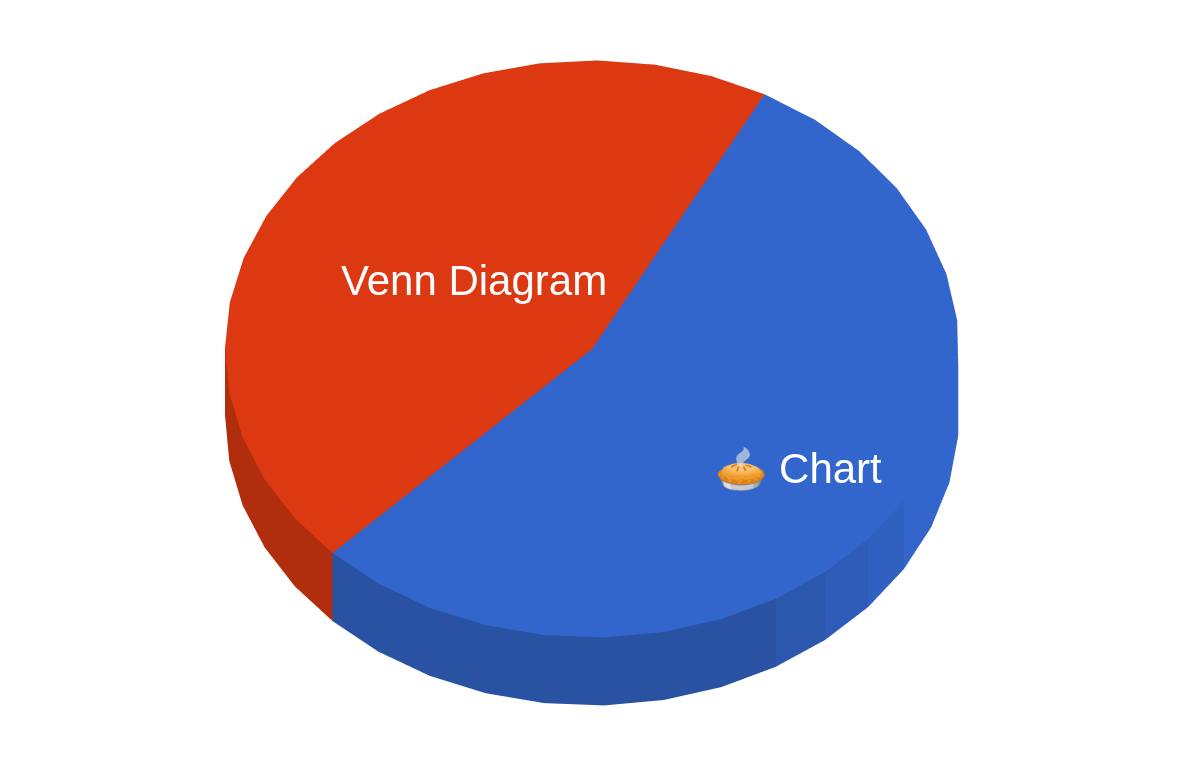
\includegraphics[width=\linewidth]{pie_charts/pie5_2005.png}
        \caption{2005}
    \end{subfigure}%
    \hfill
    \begin{subfigure}[t]{0.2\textwidth}
        \centering
        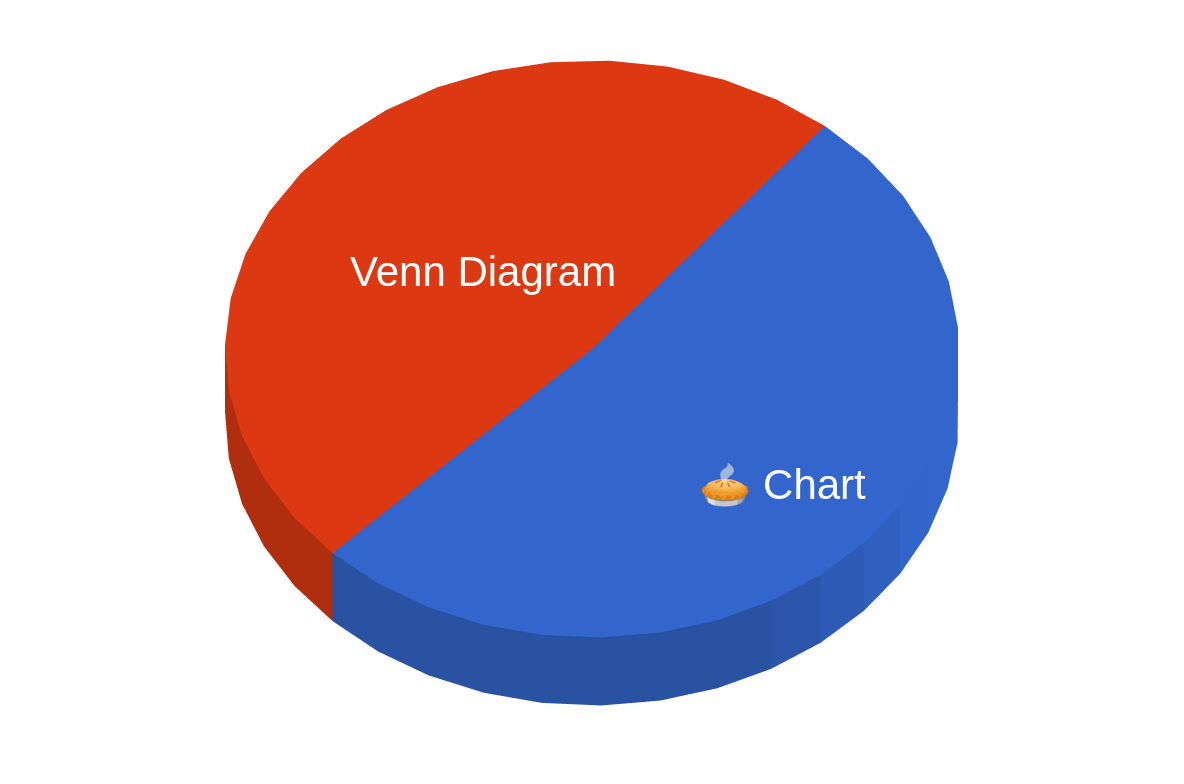
\includegraphics[width=\linewidth]{pie_charts/pie5_2010.png}
        \caption{2010}
    \end{subfigure}%
    \hfill
    \begin{subfigure}[t]{0.2\textwidth}
        \centering
        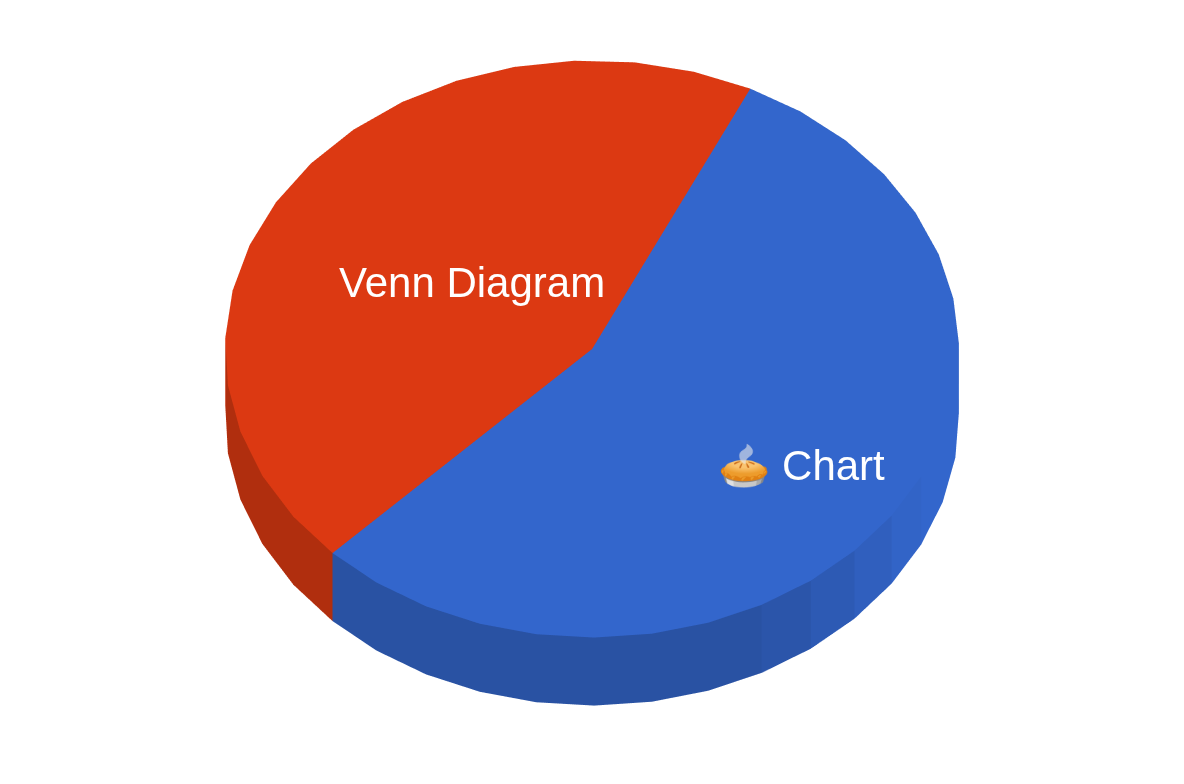
\includegraphics[width=\linewidth]{pie_charts/pie5_2015.png}
        \caption{2015}
    \end{subfigure}%
    \hfill
    \begin{subfigure}[t]{0.2\textwidth}
        \centering
        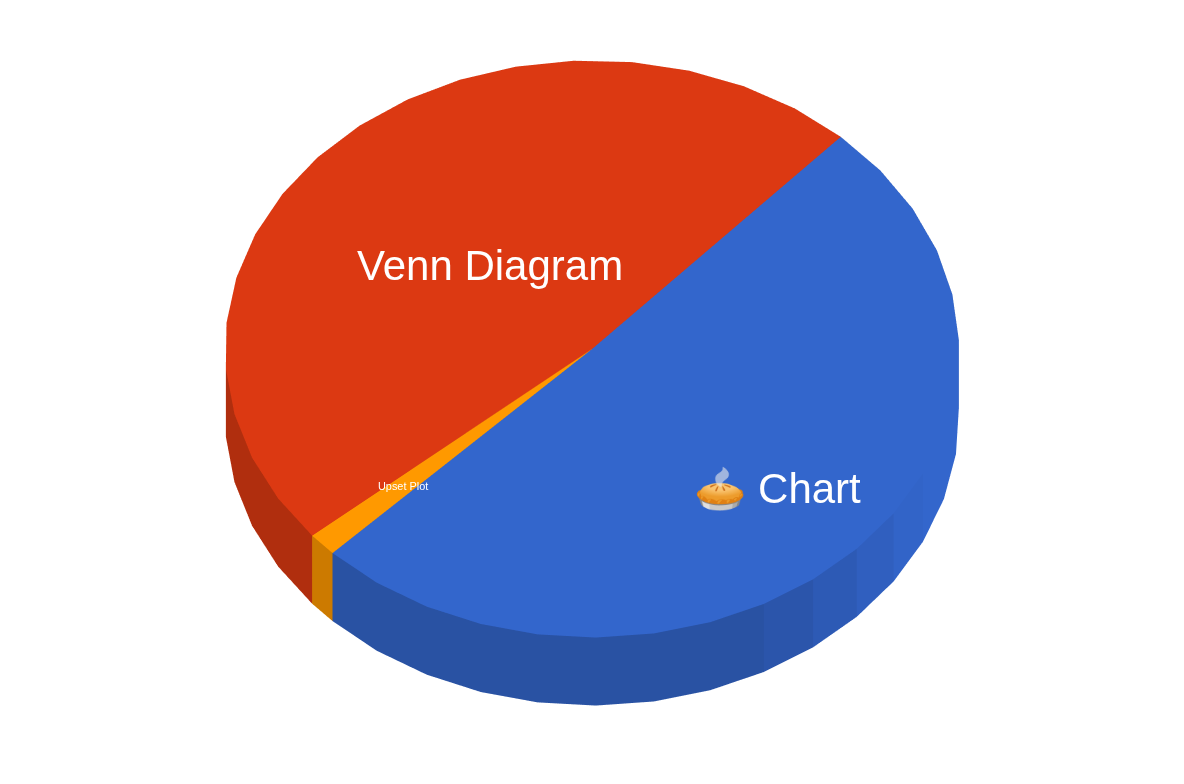
\includegraphics[width=\linewidth]{pie_charts/pie5_2020.png}
        \caption{2020}
    \end{subfigure}%
    \hfill
    \begin{subfigure}[t]{0.2\textwidth}
        \centering
        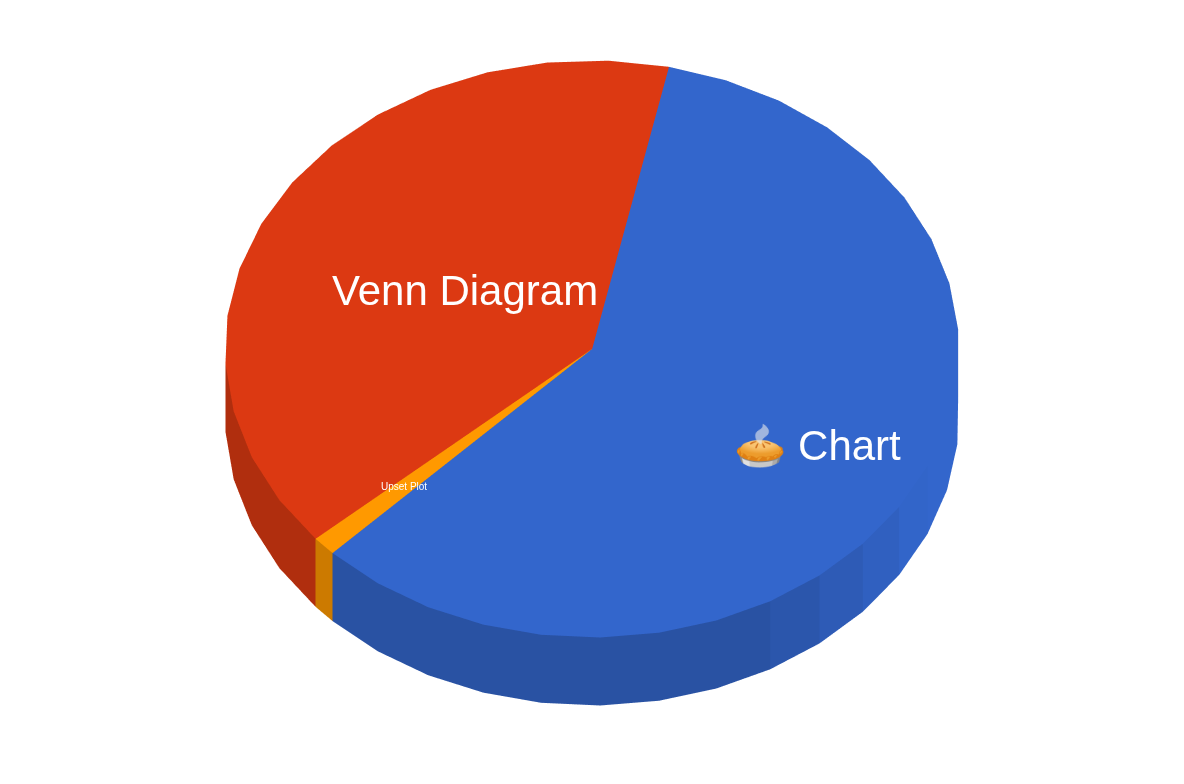
\includegraphics[width=\linewidth]{pie_charts/pie5_2025.png}
        \caption{2025}
    \end{subfigure}%
    \caption{Evolution of \pie{}chart usage compared against \venn{}s and UpSet plots, sampled in March of the years 2005, 2010, 2015, 2020, and 2025. To avoid potential influence from the holidays, when potentially more \pie{} is eaten, we decided to sample the trends in March instead of December/January.}
    \label{fig:trends}
\end{figure}

Here, we want to emphasize the striking correlation that \pie{}charts have with economic performance. No wonder it is the go-to visualization of businesspeople. 


\subsection{User Study: \pie{}charts support Calorie Intake}
\epigraph{\ldots{} as American as apple \pie{}}{}

\noindent
To test the importance of \pie{}charts in practice, we conducted a preregistered user study\footnote{\href{https://github.com/Iseratho/pieviz/blob/main/paper/userstudy/preregistration.md}{https://github.com/Iseratho/\pie{}viz/blob/main/paper/userstudy/preregistration.md}}.

First, we performed an apple \pie{} algorithm for recruitment purposes (see Algorithm~\ref{alg:applepie} in the Appendix for reproducibility). The result of the algorithm was split into 16 equal \pie{}ces used for compensation (see Figure~\ref{fig:setup}). Note that to ensure \pie{} anonymity, we overlaid the image with the compensation scheme. The authors pretested the following questionnaire so that they also earned a delicious slice of the compensation:
\begin{description}
    \item[\pie{} Affinity] Do you like \pie{}?
    \item[\pie{} Literacy] Identify the \pie{}chart among the options. Use your dessert fork to point to the visualization.
    \item[\pie{} Craving] Please allocate 3.14159 points among the following visualizations to reflect their relative impact on your appetite. A higher score indicates a stronger craving.
\end{description}
For Q2 and Q3, participants were handed a sheet containing three types of visualization (i.e., \pie{}charts, \venn{}, and UpSet plots), which we co\pie{}d from the first image of their respective Wikipedia page. To not waste the obtained information, we will include the pretest results in the evaluation. We then recruited 14 additional test subjects (i.e., colleagues) who expressed interest in tasting a slice of apple \pie{}.

\begin{figure}[H]
    \centering
    \begin{subfigure}[t]{0.5\textwidth}
        \centering
        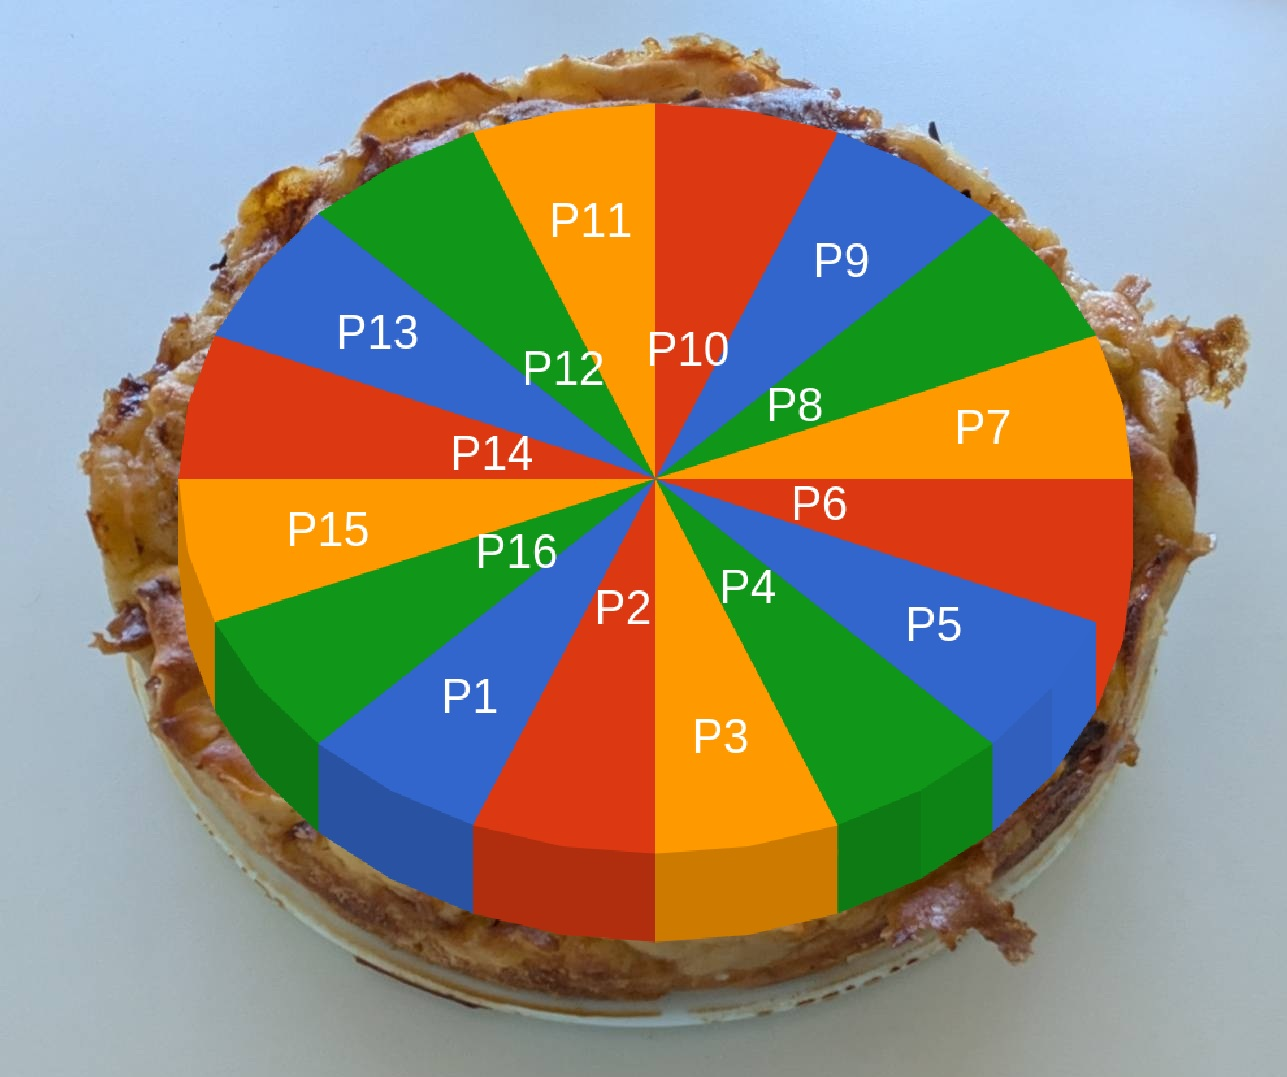
\includegraphics[width=\linewidth]{pie_charts/pie6_studysetup_anon_compensation.jpeg}
        \caption{Study Setup and Compensation}
        \label{fig:setup}
    \end{subfigure}%
    \hfill
    \begin{subfigure}[t]{0.5\textwidth}
        \centering
        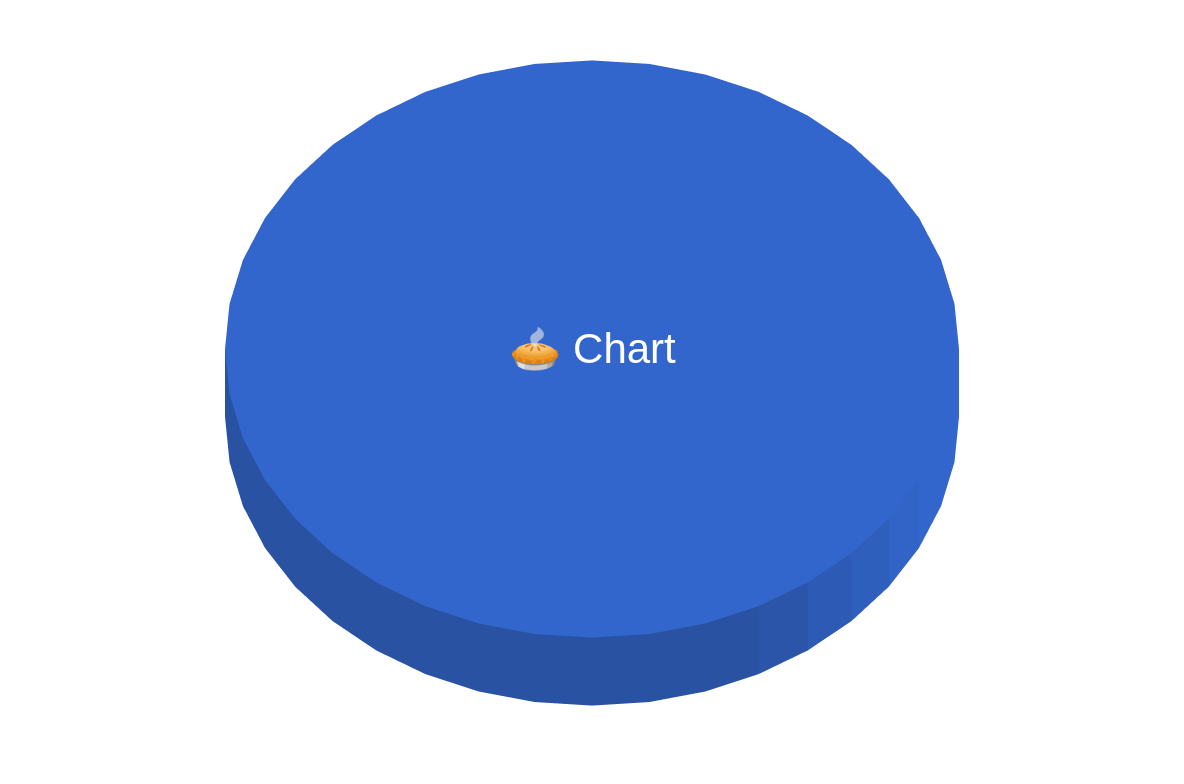
\includegraphics[width=\linewidth]{pie_charts/pie6_identified.png}
        \caption{Visualizations Identified}
        \label{fig:q2}
    \end{subfigure}%
    \hfill
    \begin{subfigure}[t]{0.5\textwidth}
        \centering
        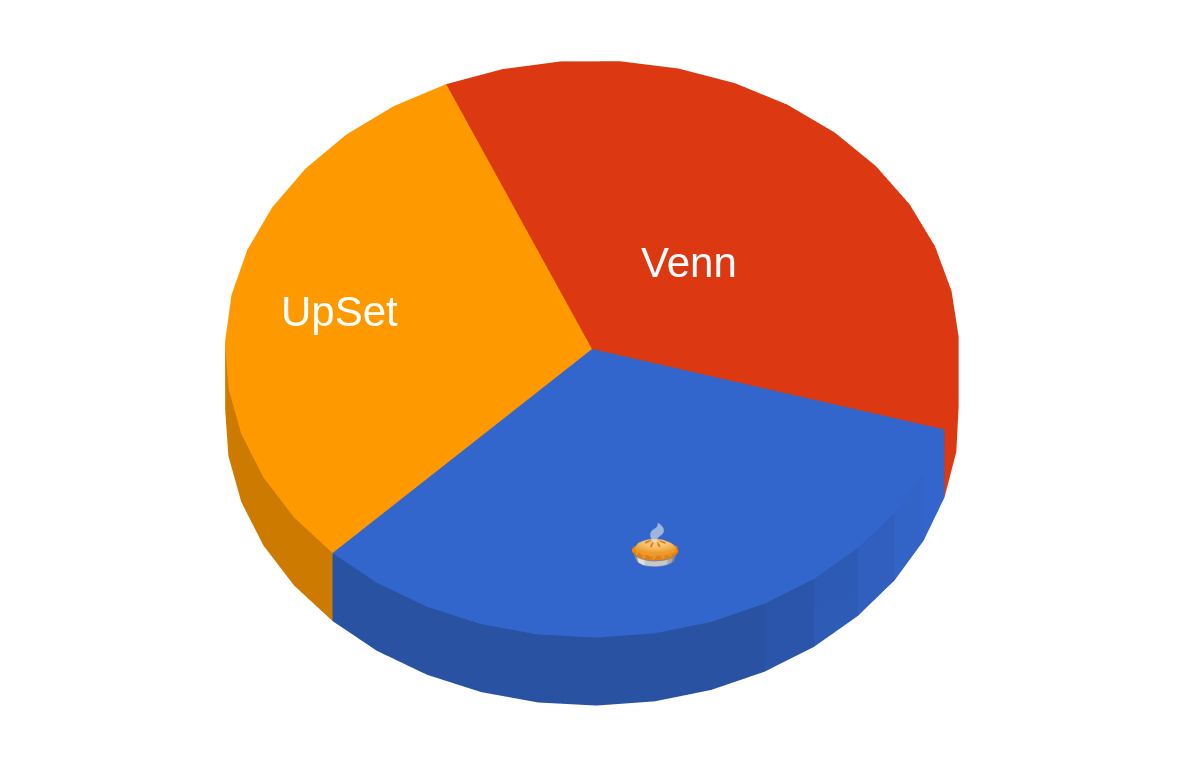
\includegraphics[width=\linewidth]{pie_charts/pie6_simulation.png}
        \caption{Random Simulation}\
        \label{fig:simulation}
    \end{subfigure}%
    \hfill
    \begin{subfigure}[t]{0.5\textwidth}
        \centering
        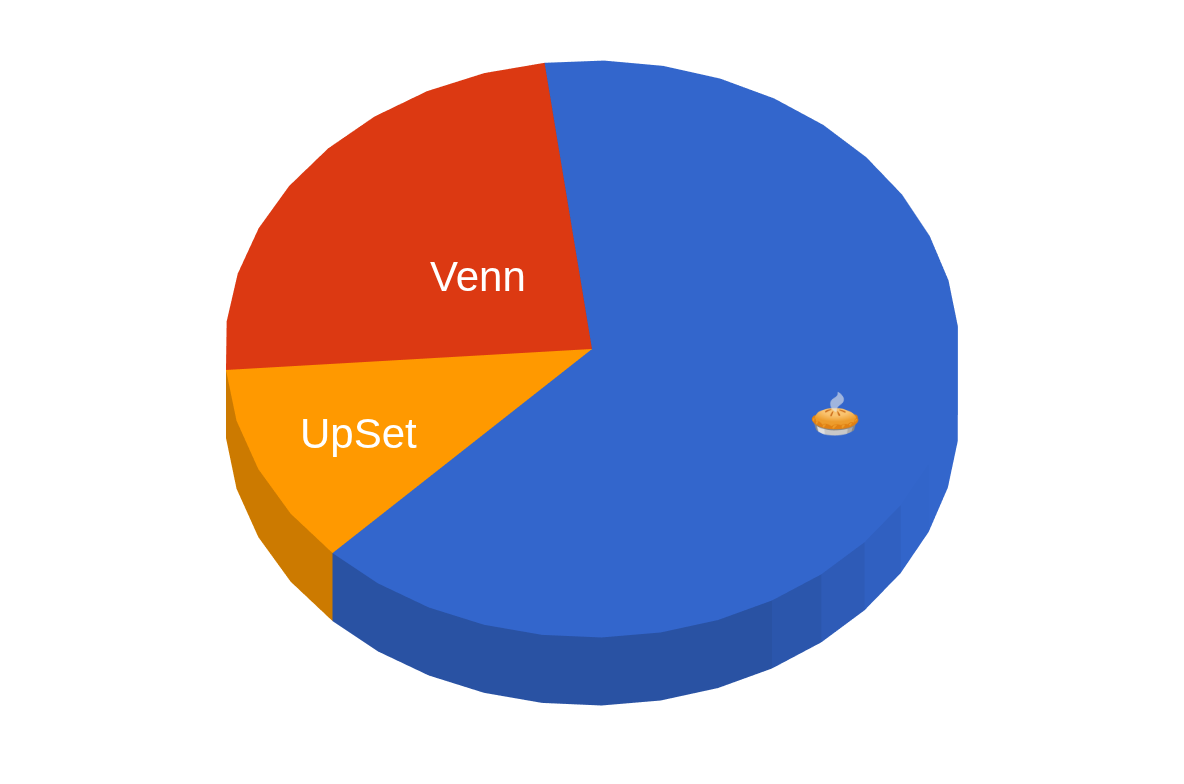
\includegraphics[width=\linewidth]{pie_charts/pie6_userstudy.png}
        \caption{Gluttonous Score}
        \label{fig:q3}
    \end{subfigure}%
    \caption{Results of the User Study. The difference between (c) and (d) is visually significant.}
    \label{fig:userstudy}
\end{figure}

We used \pie{} affinity as a screening question. Hence, we would have filtered out participants who answered no, as these weird people have obviously biased reasoning. Fortunately, every participant liked \pie{}\pie{}. The ``knowledge question'' of \pie{} literacy served multiple purposes, such as an attentiveness/manipulation check. Figure~\ref{fig:q2} shows that only the \pie{}chart was correctly identified. No participant was able to identify either the \venn{} or UpSet plot. Finally, we aggregated the points assigned for \pie{} craving to the gluttonous score. A simulation (i.e., asking an AI to assign points randomly) showed that if participants were to assign scores randomly, then the three visualizations would receive almost the same score (Figure~\ref{fig:simulation}). However, the resulting score shows the majority of points were assigned to the \pie{}chart (Figure~\ref{fig:q3}). A visual comparison reveals the significant difference between the random and actual distribution. More details and additional results can be found in Appendix~\ref{app:qualitative}.
































\section{\pie{}viz: A comprehensive \pie{}thon visualization library}
\epigraph{pip install \pie{}viz}{}
\noindent
While there are several existing libraries like matplotlib that can visualize \pie{}charts they tend to have two major oversights. First, the visualized \pie{}charts tend to be limited to boring 2D rather than awesome 3D. Second, they also support other useless types of visualizations. For that reason, we decided to create our own library \pie{}viz and released it to the public on \pie{}\pie{}\footnote{\href{https://pypi.org/project/pieviz/}{https://pypi.org/project/\pie{}viz/}}.\\ %

\fbox{%
    \parbox{\textwidth}{%
        \textbf{Sustainability Note:} To save on consuming human energy, the entire library was vibe coded. 
    }%
}\\

The library enables you to insert either a \pie{}thon dictionary or CSV file, from which a single or series of visually appealing 3D-\pie{}charts will be  created. All figures in the current paper were generated with \pie{}viz.\\

\noindent
We conducted three additional experiments to demonstrate the merits of our library:
\begin{enumerate}
    \item We benchmarked the library with an established benchmark dataset.
    \item We proved the multimodal capabilities by visualizing the semantics in complex subject matters.
    \item We demonstrate the self-referential potential, strongly suggesting \pie{} consciousness. %
\end{enumerate}
















\subsection{Benchmarking: Visualizing \pie{} in a Food-Related Dataset}
\epigraph{and now for something completely different: real research data (which contains \pie{})}{}
\noindent
We extensively evaluate our library on an established food-related benchmark dataset: Food-101~\cite{bossard14}. To that end, we visualized the \pie{} ratio with a \pie{}chart, also known as a \pie{}\pie{}chart (Figure~\ref{fig:food101}). The tiny slice of \pie{} confirms our suspicion that both nutrition and research do not contain enough \pie{}. %


\begin{figure}[h]
    \centering
    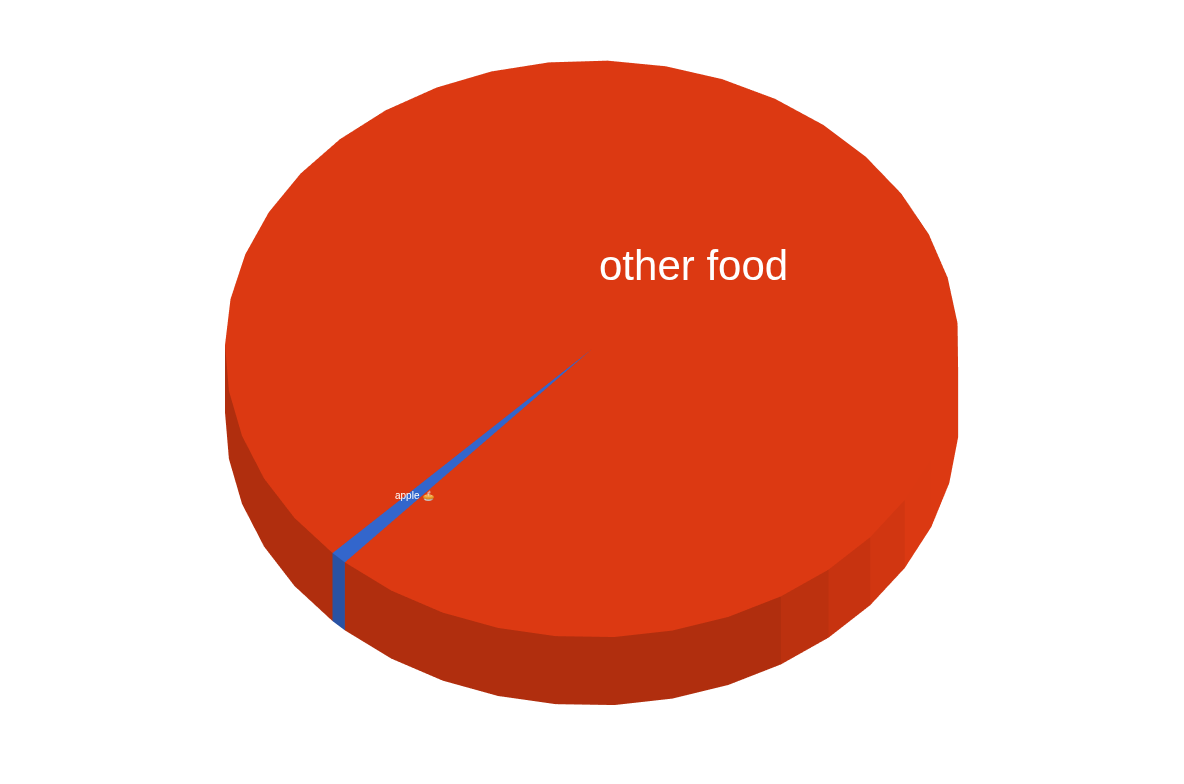
\includegraphics[width=0.5\linewidth]{pie_charts/pie7_food101.png}
    \caption{\pie{}\pie{}chart reveals the diet imbalance in the Food 101 dataset --- only a tiny \pie{} slice.}
    \label{fig:food101}
\end{figure}











\subsection{Case Study: Understanding the Meaning of Gödel, Escher, Bach with \pie{}}
\epigraph{In \pie{} we crust!}{}
\noindent
To show the capabilities in other modalities, we analyze language in Gödel, Escher, Bach~\cite{hofstadter1999godel}, which is seen as one of the most demanding books to understand due to self-referential reasoning. Figure~\ref{fig:geb} visualizes multiple occurring words in the first paragraph of the subheading ``The Self-Symbol and Free Will'' (Chapter XX). Rather than numerical Bag-of-Words representations, \pie{}charts reveal the semantics. We clearly see that the paragraph deals with the self, symbol and free, will. Moreover, we see a shift towards symbol in the later sentences. 





\begin{figure}[h]
    \centering
    \begin{subfigure}[t]{0.33\textwidth}
        \centering
        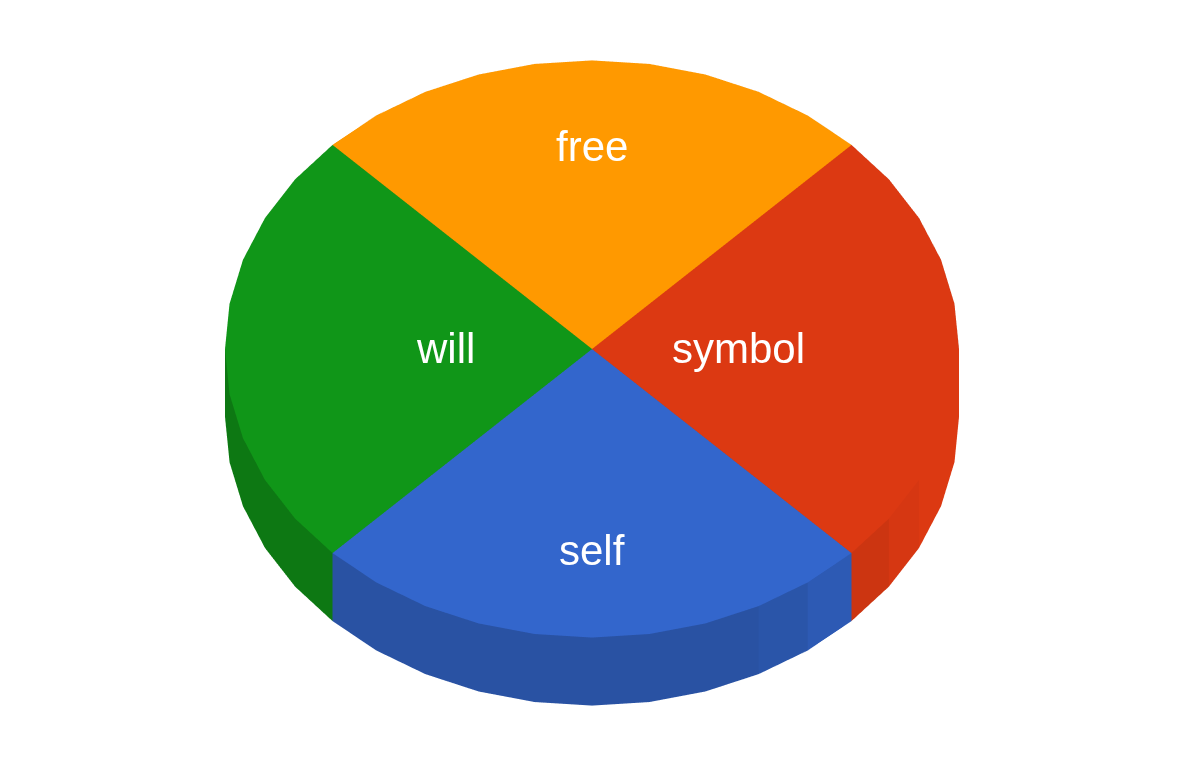
\includegraphics[width=\linewidth]{pie_charts/pie8_Heading.png}
        \caption{Heading}
    \end{subfigure}%
    \hfill
    \begin{subfigure}[t]{0.33\textwidth}
        \centering
        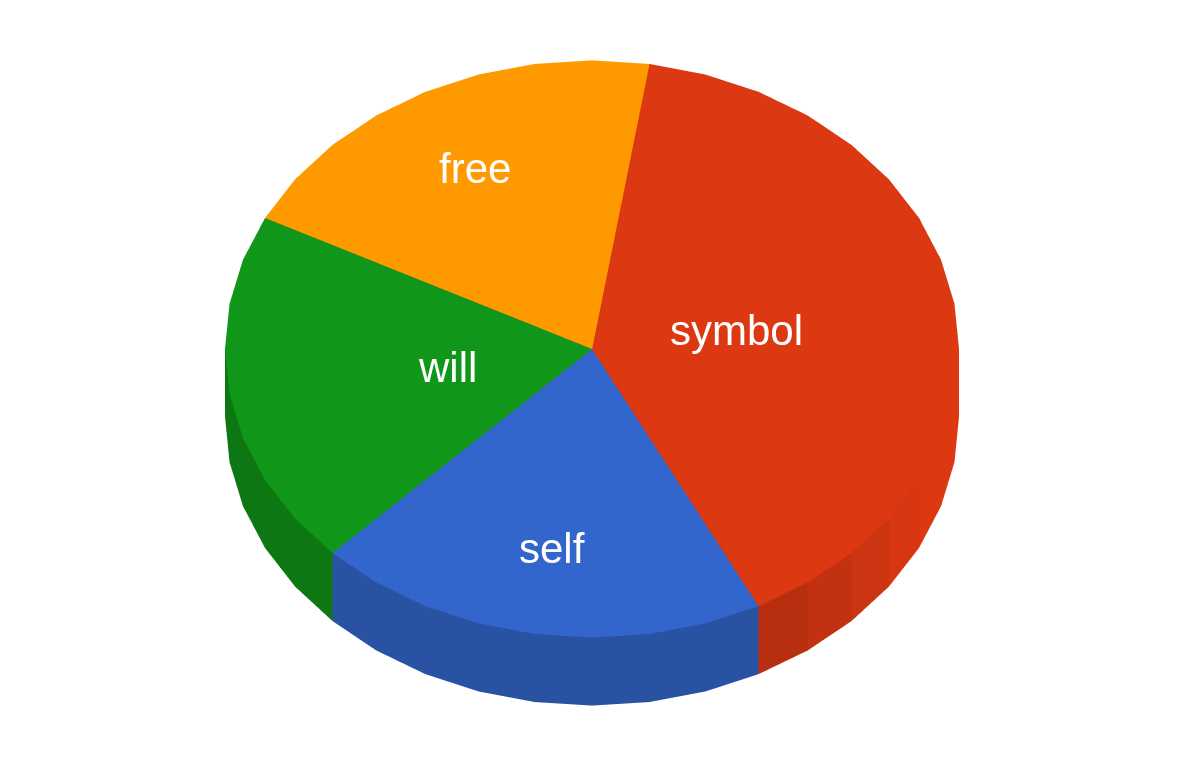
\includegraphics[width=\linewidth]{pie_charts/pie8_First.png}
        \caption{First Sentence}
    \end{subfigure}%
    \hfill
    \begin{subfigure}[t]{0.33\textwidth}
        \centering
        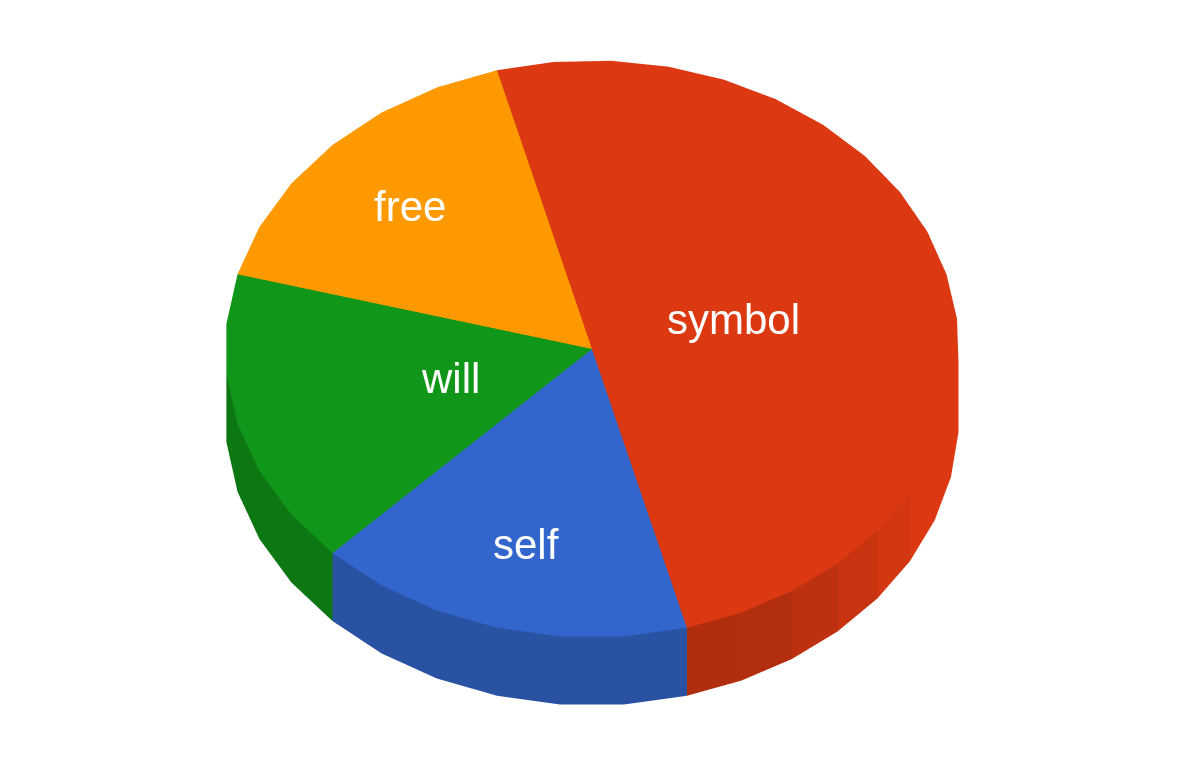
\includegraphics[width=\linewidth]{pie_charts/pie8_Second.png}
        \caption{Second Sentence}
    \end{subfigure}%
    \caption{Data Analysis of GEB to understand its meaning. We put the most prominent words into the \pie{}chart We see that the content deals with the self, symbols, and free, will. We don't need to read single sentence and observe that the story shifts towards symbols.}
    \label{fig:geb}
\end{figure}

This shows that \pie{}viz opens new directions in natural language understanding, an area previously occu\pie{}d by non-\pie{}-based visualizations.




\subsection{Recursive \pie{}: \pie{}chart analysis of \pie{}charts in a paper about \pie{}charts}
\epigraph{ \pie{} within a \pie{} within a \pie{}}{}
\noindent
Speaking of self-referential reasoning, another advantage of \pie{}charts is that they can easily reason about themselves. This is due to the ability of \pie{}charts to deal with uncertainty. Where other types of visualizations require precise numbers, you can create plausible-looking \pie{}charts with estimations. In this regard, we analyzed the color ink requirement of the current paper in Figure~\ref{fig:selfref}. Hence, we plugged in some ballpark numbers derived from the visual inspection of the paper early in the writing process. 





\begin{figure}[t]
    \centering
    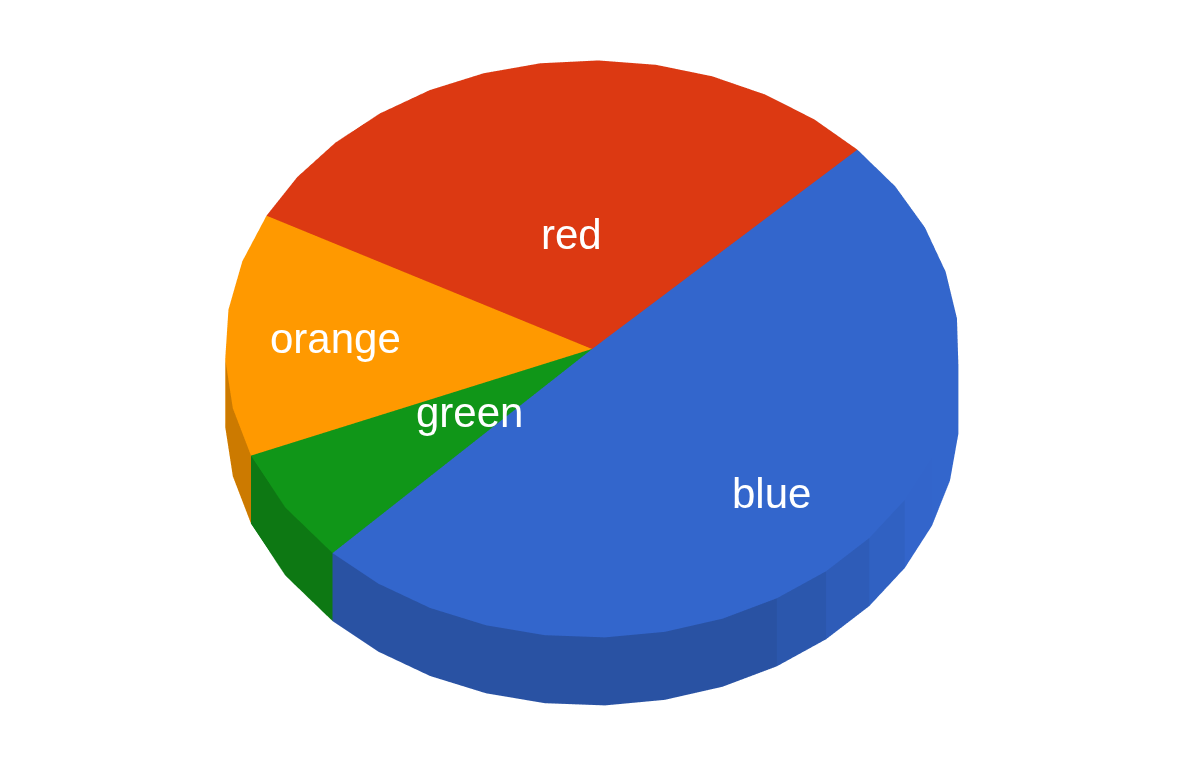
\includegraphics[width=0.5\linewidth]{pie_charts/pie9_paper_analysis.png}
    \caption{Analysis of the color ink requirements for this paper. The assessment was conducted without any measurements, and no verification of accuracy is required. }
    \label{fig:selfref}
\end{figure}

The takeaways of this analysis are threefold. First, \pie{}charts can be used to reason about \pie{}charts. This self-referential reasoning strongly hints at consciousness. We would even say that ``It may be that today's \pie{}charts are slightly conscious.'' Second, \pie{}charts enable proper data visualization for people without ANY data literacy, tremendously expanding the group of people that can create data visualizations to support their opinion with believable claims, e.g., to win arguments in online social media. Third, the \pie{}chart does not just reason over the colors of previous and its own visualization but also the colors of the figures yet to come. Hence, \pie{}charts may even be able to predict the future. 


\section{Discussion on the \pie{} Superiority}
\epigraph{The \pie{} is not a lie.}{}

\paragraph{Dismissing the Anti-\pie{} Sentiment.}
Although the evidence is clear, there is an anti-\pie{} conspiracy trying to halt the adoption of \pie{}charts - likely funded by typewriter companies to stall the visualization progress that typewriters can no longer compete with. With slogans like "the \pie{} is a lie" -- their main argument is that language is more efficient for disseminating information. Case in point, this \pie{}-based approach made it possible to finally contribute to SIGBOVIK in a very brief amount of time, which would otherwise not have been possible. Specifically, we were able to stretch what was worth not even a single page of content into a long research paper, mainly due to the efficiency of \pie{} visualizations. Not only that, writing the paper in \LaTeX was much easier, as we could put all figures into a single folder called ``\pie{}\_charts'' rather than creating elaborate folder structures for the different visualization types. This is a strong argument for how \pie{}-based visualization can accelerate research output measured in terms of published pages.



\paragraph{Conclusion: The Final Slice of \pie{}.}


In this paper, we thoroughly analyzed data visualizations that led to the preordained conclusion that \pie{}charts are superior. In sum, our first and only required point of evidence is that they have \pie{} in their name.

\noindent
Still, while working on the paper, we also found several noteworthy insights:
\begin{enumerate}
    \item Neither nutrition nor research contains enough \pie{}.
    \item \pie{}charts support calorie intake, directly addressing the UN Sustainable Development Goal 2 (SGD~2: Zero Hunger).
    \item \pie{}charts increase research output by stretching content and enabling citizen science, as no data literacy is required.
    \item \pie{}charts have a profound economic impact and are perfect for hustle culture.
\end{enumerate}
Therefore, we urgently call for a substantial rethinking of how data is presented and for people to switch entirely to \pie{} charts in (academic) publishing.


\paragraph{Limitations: Not Enough \pie{}.}
Unfortunately, academic writing uses human language rather than relying entirely on \pie{}-based visualization for dissemination. Hence, we are unable to express our thoughts to the same extent \pie{}charts would be able to do. Also, due to the original paper deadline, we were unable to conduct the user study on \pie{} day (but still reproduced Algo~\ref{alg:applepie} on 3/14).

\paragraph{Future Work: The \pie{} in the Oven.}
In this paper, we only look at the benefits of static, paper-based \pie{} visualizations. While we ensured to visualize the \pie{}charts in 3D, it still does not have the same characteristics as an actual 3D-\pie{}chart in the real world could achieve. Hence, we aim to explore the possibility of using actual \pie{}\pie{} for data visualization in the future. Such real-life representation of data would also support other sensory stimuli like haptic, smell, and taste besides just visuals. Thus, they present a way forward for data literacy of visually impaired people.

\section{Acknowledgement}

We want to specifically thank 
Apple~\pie{}, Pumpkin~\pie{}, Pecan~\pie{}, Cherry~\pie{}, Blueberry~\pie{}, Rhubarb~\pie{}, Strawberry Rhubarb~\pie{}, Key Lime~\pie{}, Lemon Meringue~\pie{}, Chocolate Silk~\pie{}, Banana Cream~\pie{}, Coconut Cream~\pie{}, Sweet Potato~\pie{}, Shepherd's~\pie{}, Chicken Pot~\pie{}, Steak and Kidney~\pie{}, Mince~\pie{}, Banoffee~\pie{}, Shoofly~\pie{}, Chess~\pie{}, Derby~\pie{}, Mud~\pie{}, Grasshopper~\pie{}, Peach~\pie{}, Blackberry~\pie{}, Raspberry~\pie{}, Marionberry~\pie{}, Boysenberry~\pie{}, Gooseberry~\pie{}, Huckleberry~\pie{}, Cranberry~\pie{}, Pear~\pie{}, Apricot~\pie{}, Plum~\pie{}, Meat~\pie{}, Pork~\pie{}, Tourtière, Fish~\pie{}, Tamale~\pie{}, Cottage~\pie{}, Pot~\pie{}, Crawfish~\pie{}, Natchitoches Meat~\pie{}, Game~\pie{}, Shaker Lemon~\pie{}, Buttermilk~\pie{}, Vinegar~\pie{}, Sugar~\pie{}, Custard~\pie{}, Egg Custard~\pie{}, Peanut Butter~\pie{}, Butterscotch~\pie{}, Caramel~\pie{}, Boston Cream~\pie{}, Whoo\pie{}~\pie{}, Moon~\pie{}, Frito~\pie{}, Pizza~\pie{}, Tomato~\pie{}, Hand~\pie{}, Fried~\pie{}, Buko~\pie{}, Ube~\pie{}, Guinness~\pie{}, Steak and Ale~\pie{}, Turkey~\pie{}, Shepherdess~\pie{}, Homity~\pie{}, Stargazy~\pie{}, Woolton~\pie{}, Pigeon~\pie{}, Squab~\pie{}, Rabbit~\pie{}, Venison~\pie{}, Aussie Meat~\pie{}, S'mores~\pie{}, Rocky Road~\pie{}, Turtle~\pie{}, Millionaire~\pie{}, Ice Cream~\pie{}, Frozen Yogurt~\pie{}, Jello~\pie{}, Kool-Aid~\pie{}, Ambrosia~\pie{}, Mock Apple~\pie{}, Mock Mincemeat~\pie{}, and all the other \pie{}\pie{}.




\bibliography{upset}
\bibliographystyle{acm}


\section*{Author Contribution Statement}

\begin{figure}[H]
    \floatbox[{\capbeside\thisfloatsetup{capbesideposition={right,top},capbesidewidth=9cm}}]{figure}[\FBwidth]
{\caption{Visualization of author contributions. We took an estimate of the contributed \pie{}-related ideas weighted by their \pie{}ness. Kevin narrowed the idea to focus solely on \pie{}charts, as well as the paper title. Markus designed the paper structure and individual experiments.
}\label{fig:authorcontiribution}}
{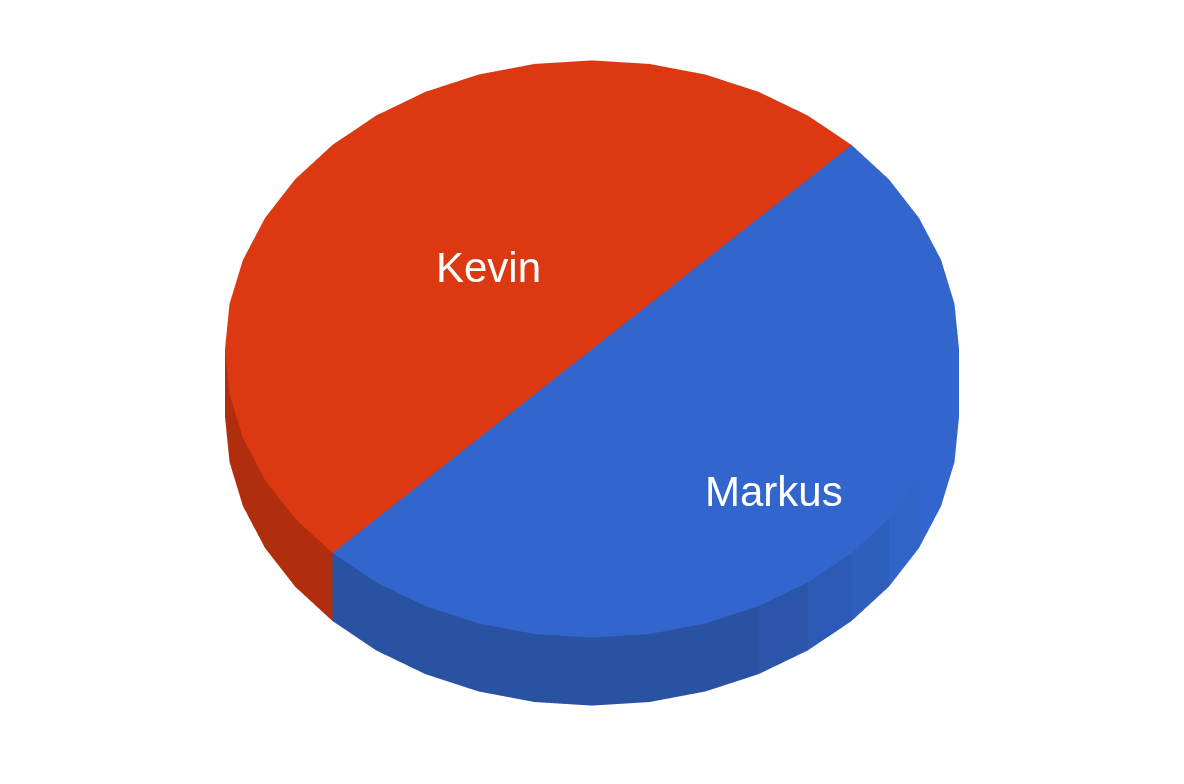
\includegraphics[width=0.75\linewidth]{pie_charts/pie10_author_contribution.png}}
\end{figure}

\renewcommand{\thesection}{\Alph{section}}
\setcounter{section}{0}

\titleformat{\section}
  {\normalfont\Large\bfseries}   %
  {Appendix \thesection{}:}         %
  {1em}                          %
  {}

\section{Additional Information on the User Study Setup}
\label{app:algorithm}

Algorithm~\ref{alg:applepie} provides the instructions for reproducing the study setup. Please note that we promote \textbf{diversity} in specified measurement units (and notations for specifying fractions).

\begin{algorithm}[h]
\caption{Apple \pie{} algorithm. }\label{alg:applepie}
\begin{algorithmic}
    \Require Butter (slightly over 1 stick)
    \Require Sugar (approximately 5/8 of a cup)
    \Require Eggs (5 and a quarter oz) \Comment{Must be from your family's farm}
    \Require Baking Soda ($1\frac{3}{4}$tsp) 
    \Require Flour ($0,\overline{5511}$ lbs)
    \Require Apples (precisely 71.5 mol) \Comment{Consider both $C_{12}H_{22}O_{11}$ and $H_{2}O$}
    \Ensure Ingredients are not spoiled
    \State Preheat oven to 360 degrees
    \State Bowl $\gets$ butter, sugar, eggs, baking soda, flour
    \While{\pie dough $\neq$ mixed}
        \State Mix(\pie dough)
    \EndWhile
    \State \pie dough $\gets$ slice(apples)
    \State Baking pan $\gets$ \pie dough
    \If{Temperature(oven) = 360°}
        \State Oven $\gets$ baking pan
        \State Sleep for 3141592ms \Comment{Safety Notice: Set an alarm to wake up on time!}
    \EndIf
    \State Enjoy while warm :-)
\end{algorithmic}
\end{algorithm}

\section{Additional Qualitative Analyses}
\label{app:qualitative}

One participant not just liked \pie{}\pie{}, but loves them (Figure~\ref{fig:pielike}). Several people complimented the \pie{}, which was standing next to them, before actually being rewarded the \pie{}ce (Figure~\ref{fig:piecompliment}). Still, the majority were stoic and able to control their urges until rewarded. Full data in \href{https://github.com/Iseratho/pieviz/tree/main/paper/userstudy}{\pie{}viz library repository}. %

\begin{figure}[h]
    \centering
    \begin{subfigure}[t]{0.5\textwidth}
        \centering
        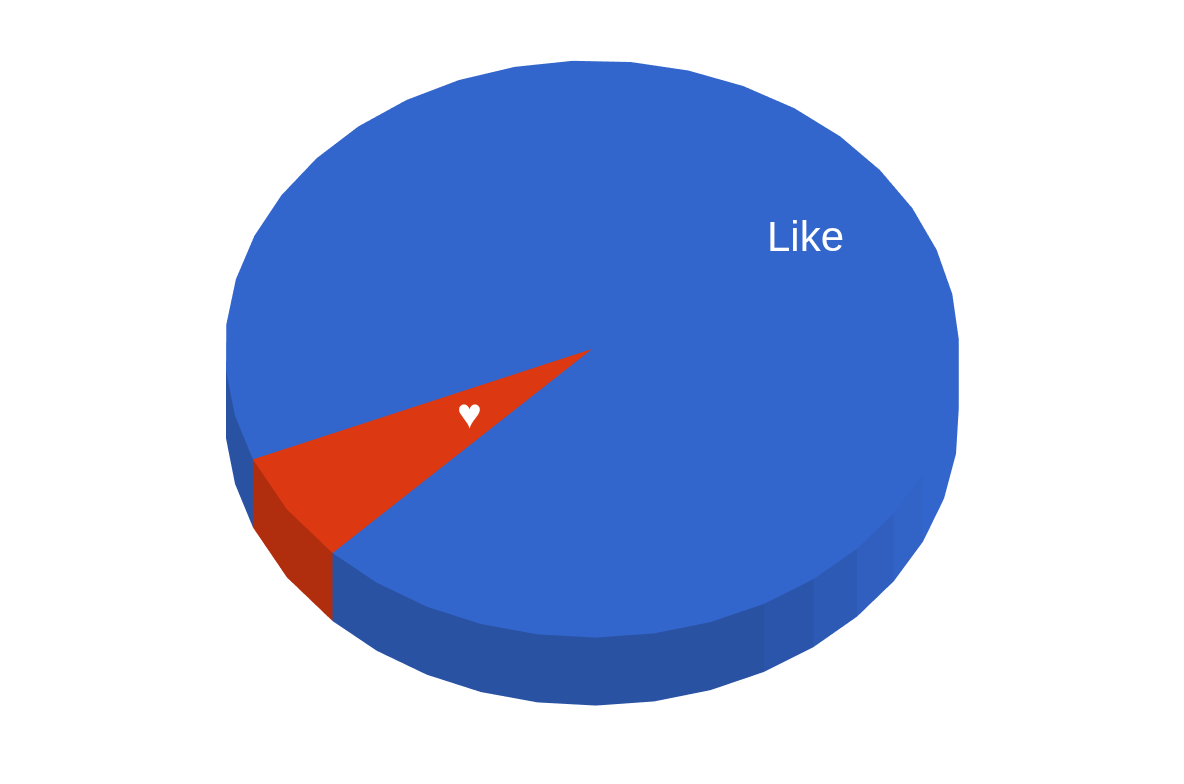
\includegraphics[width=\linewidth]{pie_charts/pie11_pielike.png}. 
        \caption{Ratio of people liking \pie{}\pie{}.}
        \label{fig:pielike}
    \end{subfigure}%
    \hfill
    \begin{subfigure}[t]{0.5\textwidth}
        \centering
        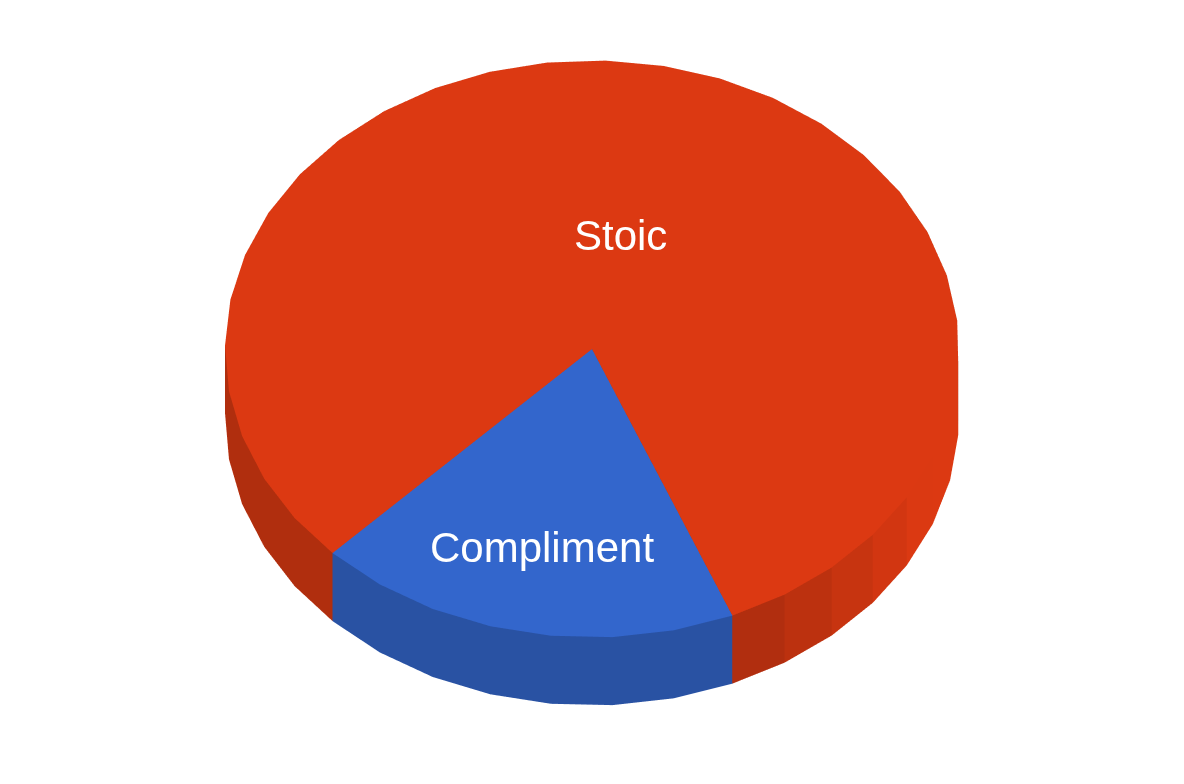
\includegraphics[width=\linewidth]{pie_charts/pie11_piecompliment.png}
        \caption{People complimenting the \pie{} before being rewarded.}
        \label{fig:piecompliment}
    \end{subfigure}%
    \caption{Additional non-preregistered analysis of the user study.}
    \label{fig:additional}
\end{figure}


\end{document}
